\documentclass[a4paper]{article}
\usepackage{pgf,tikz,pgfplots}
\usetikzlibrary{arrows,decorations.markings}
\pgfplotsset{compat=1.15}
\usepackage{mathrsfs}
\usetikzlibrary{arrows}
%% Language and font encodings
\usepackage[english]{babel}
\usepackage[utf8x]{inputenc}
\usepackage[T1]{fontenc}
\usepackage{float}
%% Sets page size and margins
\usepackage[a4paper,top=3cm,bottom=2cm,left=3cm,right=3cm,marginparwidth=1.75cm]{geometry}
\usepackage{fancyhdr}
\pagestyle{fancy}
%% Useful packages
\usepackage{tensor}
\usepackage{amsmath}
\usepackage{amsthm}
\usepackage{enumitem}
\usepackage{eqnarray}
\usepackage{float}
\usepackage{esint}
\usepackage{wrapfig}
\usepackage{gensymb}
\usepackage{lipsum}
\usepackage{amssymb}
\usepackage{array}
\usepackage{tikz}
\usepackage[colorlinks=true, allcolors=blue]{hyperref}
\usepackage{graphicx}
\usepackage{amsmath}
\usepackage{amssymb}
\usepackage{graphicx}
\usepackage[colorlinks=true, allcolors=blue]{hyperref}
\usepackage{mathtools}
\DeclareMathOperator{\Proj}{Proj}
\DeclareMathOperator{\lcm}{lcm}
\DeclareMathOperator{\cosec}{cosec}
\DeclareMathOperator{\sgn}{sgn}
\DeclareMathOperator{\Span}{span}
\DeclareMathOperator{\nullity}{nullity}
\DeclarePairedDelimiter\floor{\lfloor}{\rfloor}
\DeclareMathOperator{\Res}{Res}
\DeclareMathOperator{\rank}{rank}
\DeclareMathOperator{\Ker}{Ker}
\DeclareMathOperator{\R}{R}
\DeclareMathOperator{\Tr}{Tr}
\DeclareMathOperator{\diag}{diag}
\DeclareMathOperator{\Log}{Log}
\DeclareMathOperator{\sech}{sech}
\DeclareMathOperator{\Var}{Var}
\newtheorem{ans}{Answer}[section]
\newtheorem{defi}{Definition}[section]
\newtheorem{remarks}{Remarks}[section]
\newtheorem{note}{Note}[section]
\newtheorem{law}{Law}[section]
\newtheorem{eg}{Example}[section]
\newtheorem{notation}{Notation}[section]
\newtheorem{thm}{Theorem}[section]
\newtheorem{prop}{Proposition}[section]
\newtheorem{lemma}{Lemma}[section]
\newtheorem{cor}{Corollary}[section]
\definecolor{darkblue}{RGB}{	0, 0, 139}
\newtheoremstyle{new}% <name>
{2pt}% <Space above>
{2pt}% <Space below>
{\color{darkblue}}% Body font
{}% <Indent amount>
{\bfseries\color{black}}% Theorem head font
{:}% <Punctuation after theorem head>
{.5em}% <Space after theorem headi>
{}% <Theorem head spec (can be left empty, meaning `normal')>
\theoremstyle{new}
\newtheorem{qns}{Problem}[section]
\setlength{\parindent}{0cm}
\title{\textbf{Part II TP1 (Theoretical Physics 1)}}
\author{Tai Yingzhe, Tommy (ytt26)}
\date{}
\setlength{\parindent}{0cm}
\begin{document}
\maketitle
\tableofcontents
\newpage
\section{Lagrangian and Hamiltonian Mechanics}
\subsection{Lagrangian Formalism}
\subsubsection{Generalized Coordinates}
While Newtonian mechanics uses vectors, the Lagrangian approach is more flexible. A system with $n$ degrees of freedom requires $n$ independent generalized coordinates $q_i(t)$, $i=1$, ..., $n$, to specify its configuration. The generalized velocities are $\dot{q}_i=\frac{dq_i}{dt}$. Why do we do this? This is useful
\begin{itemize}
    \item in non-Cartesian coordinates, for example, polar coordinates for problems with circular or spherical symmetry. 
    \item for systems with constraints, for example, confining surfaces, curves, strings, rods, etc.
\end{itemize}
\begin{defi}[Lagrangian Mechanics]
Lagrangian mechanics deals mostly with systems that are conservative (ideal, non-dissipative). Their dynamics can be derived from a scalar function, the Lagrangian $\mathcal{L}(\mathbf{q},\mathbf{\dot{q}},t)$ where $\mathbf{q}$ stands for $(q_1,...,q_n)$ and $\mathbf{\dot{q}}$ stands for $(\dot{q}_1,...,\dot{q}_n)$, $\frac{\partial\mathcal{L}}{\partial\mathbf{q}}$ stands for $(\frac{\partial\mathcal{L}}{\partial q_1},...,\frac{\partial\mathcal{L}}{\partial q_n})$, $\mathbf{q}\cdot\mathbf{p}=q_ip_i$, etc.
\end{defi}
\subsubsection{Hamilton's Principle}
\begin{defi}[Action]
If a system evolves from an initial configuration $\mathbf{q_1}=\mathbf{q}(t_1)$ to a final configuration $\mathbf{q_2}=\mathbf{q}(t_2)$, the action is defined as a functional of the path $\mathbf{q}(t)$ taken in configuration space.
$$S[\mathbf{q}]=\int_{t_1}^{t_2}\mathcal{L}(\mathbf{q},\mathbf{\dot{q}},t)dt$$
\end{defi}
\begin{defi}[Hamilton's principle]
The Hamilton's principle states that the physical path is such that the action has a stationary value, i.e. the first variation $\delta S=\delta\int\mathcal{L}dt=0$, subject to $\mathbf{q}(t_1)$ and $\mathbf{q}(t_2)$ being fixed. 
\end{defi}
\begin{prop}
Hamilton's principle require the Lagrangian to satisfy the Euler-Lagrange equation for the variable $q_i$.
$$\frac{\partial\mathcal{L}}{\partial q_i}-\frac{d}{dt}\frac{\partial\mathcal{L}}{\partial\dot{q}_i}=0$$
\end{prop}
\begin{proof}
According to the calculus of variations (See IB Variational Principles), Hamilton's Principle mean that the functional derivative vanishes, i.e. $\frac{\partial S}{\partial q_i}=0$ for each $i=1,...,n$. This is the Euler-Lagrange equation for the variable $q_i$. The variation $\delta$ commutes with integration and differentiation. Also, $\delta\int\mathcal{L}dt=\int\delta\mathcal{L}dt$, and $\delta(\dot{q}_i)=\frac{d}{dt}(\delta q_i)=\delta\dot{q}_i$. We have
$$\delta S=\int_{t_1}^{t_2}\delta\mathcal{L}dt=\int_{t_1}^{t_2}\sum_{i=1}^n\bigg(\frac{\partial\mathcal{L}}{\partial q_i}\delta q_i+\frac{\partial\mathcal{L}}{\partial\dot{q}_i}\delta\dot{q}_i\bigg)dt=\int_{t_1}^{t_2}\sum_{i=1}^n\bigg(\frac{\partial\mathcal{L}}{\partial q_i}+\frac{d}{dt}\frac{\partial\mathcal{L}}{\partial q_i}\bigg)\delta q_idt+\bigg[\sum_{i=1}^n\frac{\partial\mathcal{L}}{\partial\dot{q}_i}\delta q_i\bigg]_{t_1}^{t_2}$$
If $\delta S$ is to vanish for all variations $\delta q_i$ and vanish at the endpoints, then we obtain the Euler-Lagrange equations.
\end{proof}
\begin{remarks}
In analytical mechanics, we call these the Lagrange's equations and interpret them as the equations of motion of the system:
$$\frac{d}{dt}\frac{\partial\mathcal{L}}{\partial\dot{q}_i}=\frac{\partial\mathcal{L}}{\partial q_i}\iff\frac{d}{dt}\frac{\partial\mathcal{L}}{\partial\mathbf{\dot{q}}}=\frac{\partial\mathcal{L}}{\partial\mathbf{q}}$$
Since $\mathcal{L}$ depends on $\mathbf{q}$ and $\mathbf{\dot{q}}$, these are $n$ second order ODEs for $q_i(t)$. In general, they are non-linear. We can identify the LHS of Lagrange equations as $\frac{dp_i}{dt}$ where $p_i=\frac{\partial\mathcal{L}}{\partial\dot{q}_i}$ is the generalized momentum, associated with the generalized coordinate $q_i$, i.e. conjugate to $q_i$.
\end{remarks}
\begin{prop}
Lagrangian is unique up to a constant and a function independent of $\dot{q}$.
\end{prop}
\begin{proof}
The constant case is obvious. Add $\frac{d}{dt}f(\mathbf{q},t)$ to $\mathcal{L}$ will render the LHS unchanged since 
$$\frac{d}{dt}f(\mathbf{q},t)=\frac{\partial f}{\partial t}+\frac{\partial f}{\partial\mathbf{q}}\cdot\mathbf{\dot{q}}$$
Then we add to $S=\int\mathcal{L}dt$, the quantity $f(\mathbf{q},t_2)-f(\mathbf{q},t_1)$ which is independent of the path. Indeed, the extra terms in the Lagrange equations cancel out.
\end{proof}
\subsubsection{Constraints}
Often we deal with systems of particles whose motion is constrained. 
\begin{eg}
For example, in a rigid body, $|\mathbf{r_i}-\mathbf{r_j}|$ is a constant $\forall i,j$, i.e. any pair of particles. In another example, in a simple pendulum, the particle can only move on a 1D circle. Forces of constraint are required to enforce these conditions. In the Newtonian approach, we introduce these forces explicitly and eliminate them algebraically. The Lagrangian method handles them more easily.
\end{eg}
\begin{prop}
Consider a system of $N$ particles moving in $\mathcal{D}$-dimensions, subject to $M$ independent holonomic constraints of the form 
$$f_m(\mathbf{r_1},...,\mathbf{r_N},t)=0$$
for $m=1,...,M$. The constraints restrict the possible configurations to a surface in $\mathbb{R}^{\mathcal{D}N}$ of dimension $n=\mathcal{D}N-M$, called the configuration space (or manifold) of this constrained system. The resulting system has $n$ degrees of freedom.
\end{prop}
\begin{defi}[Scleronomic, rhenomic constraints]
Scleronomic constraints do not depend explicitly on time, while the rheonomic constraints do. 
\end{defi}
\begin{eg}
A particle in 3D confined to move along a moving wire, is subject to two rheonomic constraints and has one degree of freedom. 
\end{eg}
\begin{prop}
The Euler-Lagrange equations with constraints $f_m(\mathbf{r_1},\dots,\mathbf{r_N},t)=0$ are
$$\frac{d}{dt}\frac{\partial\mathcal{L}}{\partial\mathbf{\dot{r}_i}}-\frac{\partial\mathcal{L}}{\partial\mathbf{r_i}}-\sum_{i=1}^M\lambda_m\frac{\partial f_m}{\partial\mathbf{r_i}}$$
for the $i$th particle. The last term is associated with forces of constraint, which can be eliminated algebraically as in the Newtonian method.
\end{prop}
\begin{proof}
To enforce $f_m=0$ at every instant $t\in(t_1,t_2)$, we require a time-dependent Lagrange multiplier $\lambda_m(t)$. The variation of action $\int\mathcal{L}dt$ is thus subject to the constraints $f_m=0$. This is equivalent to an unconstrained variation of 
$$\int(\mathcal{L}-\sum_{m=1}^M\lambda_m(t)f_m)dt=0$$
This gives the modified Lagrange equations for the $i$th particle. 
\end{proof}
\begin{prop}
A better approach is to solve the equations of constraint by introducing $n$ (dimension of configuration space) independent generalized coordinates $\{q_1,...,q_n\}$ that uniquely specify the configuration subject to all constraints. We can then write $\mathbf{r_i}(\mathbf{q})$ and $\mathbf{r_i}(\mathbf{q},t)$ for scleronomic and rheonomic constraints. For each $i=1,...,n$, we obtain the unmodified Lagrange equations
$$\frac{d}{dt}\frac{\partial\mathcal{L}}{\partial\dot{q}_i}=\frac{\partial\mathcal{L}}{\partial q_i}$$
because the $f_m$ do not depend on $q_1,...,q_n$.
\end{prop}
\begin{eg}
Consider a 2D simple pendulum of length $l$. The constraints $f=|\mathbf{r}|-l=0$ produces a force of constraint $-\lambda\boldsymbol{\nabla}f=-\lambda\frac{\mathbf{r}}{|\mathbf{r}|}$. Here, $\lambda$ is the tension in the string, or the normal reaction from a surface, required to constrain the particle to a circle. If instead of $(x,y)$, we use the generalized coordinate $\theta$, we can just solve $\frac{d}{dt}\frac{\partial\mathcal{L}}{\partial\dot{\theta}}=\frac{\partial\mathcal{L}}{\partial\theta}$ and ignore the constraint.
\end{eg}
\begin{eg}
Examples of non-holonomic constraints: inequalities, for example, particle bouncing on a table, i.e. $z\geq0$, non-integrable constraints involving velocities, for example, a sphere or a disc rolling on a surface. Surprisingly, for the case of a cylinder, the problem is integrable.
\end{eg}
\subsubsection*{Symmetries and Conservation Laws}
\begin{defi}[Cyclic coordinate]
If $\mathcal{L}$ does not depend on a particular coordinate, then that coordinate is ignorable and is known as a cyclic coordinate.
\end{defi}
\begin{thm}[Conservation of momentum]
If the Lagrangian $\mathcal{L}$ does not depend on a generalized coordinate $q_k$, then the conjugate momenta $p_k:=\frac{\partial\mathcal{L}}{\partial\dot{q}_k}$ is constant in time.
\end{thm}
\begin{proof}
Lagrange's equations for $q_k$ then reduces to $\frac{d}{dt}\frac{\partial\mathcal{L}}{\partial\dot{q}_k}=0$ which implies the conservation law: $\frac{\partial\mathcal{L}}{\partial\dot{q}_k}:=p_k$, the conjugate momenta, is constant in time.
\end{proof}
\begin{thm}[Conservation of energy]
If the Lagrangian $\mathcal{L}$ does not depend explicitly on time, then the energy is conserved.
\end{thm}
\begin{proof}
The total time derivative of $\mathcal{L}(\mathbf{q},\mathbf{\dot{q}},t)$ is, by the chain rule:
$$\frac{d\mathcal{L}}{dt}=\sum_{i=1}^N\bigg(\frac{\partial\mathcal{L}}{\partial q_i}\dot{q}_i+\frac{\partial\mathcal{L}}{\partial\dot{q}_i}\ddot{q}_i\bigg)+\frac{\partial\mathcal{L}}{\partial t}$$
If $\mathcal{L}$ does not depend explicitly on time, the last term vanishes. Using the Lagrange's equations, we then find
$$\frac{d\mathcal{L}}{dt}=\sum_{i=1}^n\bigg\{\bigg[\frac{d}{dt}\frac{\partial\mathcal{L}}{\partial\dot{q}_i}\bigg]\dot{q}_i+\frac{\partial\mathcal{L}}{\partial\dot{q}_i}\ddot{q}_i\bigg\}=\frac{d}{dt}\sum_{i=1}^N\frac{\partial\mathcal{L}}{\partial\dot{q}_i}\dot{q}_i$$
Hence, we obtain the Beltrani identity:
$$\frac{d}{dt}\bigg[\sum_{i=1}^N\frac{\partial\mathcal{L}}{\partial\dot{q}_i}\dot{q}_i-\mathcal{L}\bigg]=0$$
We need to have $\sum_{i=1}^N\frac{\partial\mathcal{L}}{\partial\dot{q}_i}\dot{q}_i-\mathcal{L}$ is a constant, which is time. Consider $\mathcal{L}=T-V$ where $T$ is now a homogeneous quadratic function of $\mathbf{\dot{q}}$ and may depend on $\mathbf{q}$ and $V$ is only a function of $\mathbf{q}$. Then, by Euler's Theorem on homogeneous functions,
$$\sum_{i=1}^n\dot{q}_i\frac{\partial T}{\partial q_i}=2T$$
We thus have $2T-\mathcal{L}=2T-(T-V)=T+V=E$, a constant. 
\end{proof}
\newpage
\begin{qns}
A uniform circular disc of mass $2m$ and radius $a$ is mounted on an axle through its centre so that it can rotate without friction in a vertical plane. A point mass $m$ is fixed at point P on the lower edge of the disc. A light elastic string with force constant $k$ is also attached to $P$, runs over the circumference of the disc without friction, passes the topmost point and hangs down vertically. At the bottom end of the string a mass $0.5m$ is attached.
\begin{figure}[H]
    \centering
    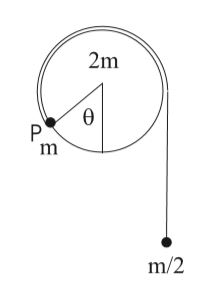
\includegraphics[scale=0.5]{Q1.JPG}
\end{figure}
Write down the Lagrangian for the system in terms of angle of rotation $\theta$ of the disc and the extension $x$ of the string with respect to its natural length. Obtain Lagrange's equation of motion.\\[5pt]
Find the equilibrium position of the disc $\theta_0$ and equilibrium extension $x_0$.\\[5pt]
Show that the natural frequencies $\omega$ of small oscillations of the system are determined by the solution to the equation
$$m^2\omega^4-\bigg(\frac{5k}{2}+\frac{\sqrt{3}mg}{4a}\bigg)m\omega^2+\frac{\sqrt{3}mgk}{2a}=0$$
For the limiting case of a stiff string ($k>>\frac{mg}{a}$), show that the natural frequencies approach $\omega^2=\frac{5k}{2m}$ and $\omega^2=\frac{\sqrt{3}g}{5a}$, and describe the normal modes.\\[5pt]
Find appropriate expressions for the other limiting case $k<<mg/a$ and interpret your results.
\end{qns}
\begin{ans}
Let $x$ is the extension of string with respect to natural length. The kinetic energy is
$$T=\frac{1}{2}\frac{1}{2}(2m)a^2\dot{\theta}^2+\frac{1}{2}ma^2\dot{\theta}^2+\frac{1}{4}m(\dot{x}+a\dot{\theta})^2=\frac{5}{4}ma^2\dot{\theta}^2+\frac{1}{4}m\dot{x}^2+\frac{1}{2}m\dot{x}a\dot{\theta}$$
where the moment of inertia of the disc is $\frac{1}{2}2ma^2$. The potential energy is
$$V=-mga\cos\theta-\frac{1}{2}mg(x+a\theta)+\frac{1}{2}kx^2$$
$$\mathcal{L}=T-V=\frac{5}{4}ma^2\dot{\theta}^2+\frac{1}{4}m\dot{x}^2+\frac{1}{2}m\dot{x}a\dot{\theta}+mga\cos\theta+\frac{1}{2}mg(x+a\theta)-\frac{1}{2}kx^2$$
We have the equations of motion
$$\frac{d}{dt}\frac{\partial\mathcal{L}}{\partial\dot{\theta}}=\frac{d}{dt}(2.5ma^2\dot{\theta}+\frac{1}{2}ma\dot{x})=2.5ma^2\ddot{\theta}+0.5ma\ddot{x},\quad\frac{\partial\mathcal{L}}{\partial\theta}=-mga\sin\theta+\frac{1}{2}mga$$
$$\frac{\partial\mathcal{L}}{\partial x}=0.5mg-kx,\quad\frac{d}{dt}\frac{\partial\mathcal{L}}{\partial\dot{x}}=0.5m\ddot{x}+0.5ma\ddot{\theta}$$
The Lagrange's equations of motion give
\begin{equation}
2.5ma^2\ddot{\theta}+0.5ma\ddot{x}=0.5mga-mga\sin\theta\tag{1a}
\end{equation}
\begin{equation}
0.5mg-kx=0.5m\ddot{x}+0.5ma\ddot{\theta}\tag{1b}
\end{equation}
The equilibrium $\ddot{\theta}=\ddot{x}=0$, so $x_0=\frac{mg}{2k}$ and $\sin\theta_0=0.5\implies\theta_0=\pi/6$.\\[5pt]
Consider small perturbation from equilibrium, i.e. $\theta=\theta_0+\delta\theta$, $x=x_0+\delta x$ and using small angle approximation, 1a and 1b respectively give
$$2.5ma^2\delta\ddot{\theta}+0.5ma\delta\ddot{x}=0.5mga-mga\sin(\theta_0+\delta\theta)\approx0.5mga-mga(0.5+0.5\sqrt{3}\delta\theta)$$
$$0.5mg-kx_0-k\delta x=0.5m\delta\ddot{x}+0.5ma\delta\ddot{\theta}$$
Assume $\delta\theta$ and $\delta x$ vary with time as $e^{i\omega t}$, $\delta\ddot{x}=-\omega^2\delta x$, $\delta\ddot{\theta}=-\omega^2\delta\theta$, so
$$\begin{pmatrix}-0.5m\omega^2+k&-0.5ma\omega^2\\-0.5ma\omega^2&-2.5ma^2\omega^2+0.5\sqrt{3}mga\\\end{pmatrix}\begin{pmatrix}\delta x\\\delta\theta\\\end{pmatrix}=0$$
Setting the determinant to be zero, 
$$0=(-0.5m\omega^2+k)(-2.5ma^2\omega^2+0.5\sqrt{3}mga)-0.25m^2a^2\omega^4=m^2\omega^4-m\omega^2\bigg(2.5k+\frac{\sqrt{3}mg}{4a}\bigg)+\frac{\sqrt{3}mgk}{2a}$$
where $m(\omega_1^2+\omega_2^2)=\frac{5k}{2}+\frac{\sqrt{3}mg}{4a}$, $m^2\omega_1^2\omega_2^2=\frac{\sqrt{3}}{2}\frac{mgk}{a}$. When $k>>mg/a$,
$$m(\omega_1^2+\omega_2^2)\approx2.5k,\quad m^2\omega_1^2\omega_2^2<<1$$
If $m\omega_2^2\approx2.5k$, then $m\omega_1^2\approx\frac{\sqrt{3}mgk}{2a}\frac{2}{5k}=\frac{\sqrt{3}mg}{5a}$. When $k<<mg/a$,
$$m(\omega_1^2+\omega_2^2)\approx\frac{\sqrt{3}mg}{4a},\quad m^2\omega_1^2\omega_2^2>>1$$
If $m\omega_2^2\approx\frac{\sqrt{3}mg}{4a}$, then $m\omega_1^2\approx\frac{\sqrt{3}mgk}{2a}\frac{4a}{\sqrt{3}mg}=2k$. 
\end{ans}
\begin{qns}
A Lagrangian explicitly dependent on time: the inverted pendulum. The system consists of a bob of mass $m$ at the far end of a light rod of length $l$ whose near end is freely hinged to a support that vibrates vertically with amplitude $a$ and frequency $\frac{\omega}{2\pi}$. Show that
$$\mathcal{L}=\frac{1}{2}m(l^2\dot{\theta}^2+\omega^2a^2\sin^2\omega t+2\omega al\sin\omega t\sin\theta\dot{\theta})-mg(a\cos\omega t+l\cos\theta)$$
where $\theta$ is the inclination to the vertical, and hence that the equation of motion is
$$l^2\ddot{\theta}+\omega^2al\cos\omega t\sin\theta-gl\sin\theta=0$$
\begin{figure}[H]
    \centering
    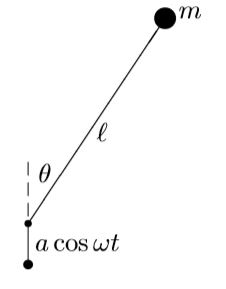
\includegraphics[scale=0.5]{Q2.JPG}
\end{figure}
The motion must consist of a `slow' ($\tau<2\pi\sqrt{l/g}$) motion and a small but forced wobble at frequency $\omega/2\pi>>1/\tau$ (and possibly harmonics). Write
$$\theta=\theta_1+C\cos\omega t+S\sin\omega t$$
where $\theta_1$, $S$ and $C$ vary slowly.\\[5pt]
Substitute this expression into the equation of motion, keeping only first order terms in the small quantities $C$ and $S$. You can then isolate the `slow' terms and those that vary at frequency $\frac{\omega}{2\pi}$; show that the latter obey
$$l^2\ddot{S}-2\omega l^2\dot{C}-\omega^2l^2S-glS\cos\theta_1=0$$
$$l^2\ddot{C}+2\omega l^2\dot{S}-\omega^2l^2C-glC\cos\theta_1=-\omega^2al\sin\theta_1$$
Near an equilibrium value of $\theta_1$, $C$ and $S$ vary arbitrarily slowly, so you can investigate the stability of, and small oscillations about an equilibrium $\theta_1$ neglecting terms in $\dot{C}$ etc. Use the resulting expressions for $C$ and $S$ in the `slow' terms of the equation of motion to show that the upright position of the pendulum is stable iff 
$$\omega^2>\frac{2gl}{a^2}$$
and find the period of small oscillations of $\theta_1$ about zero.
\end{qns}
\begin{ans}
Set the origin such that the position coordinate for the mass $m$ is $x=l\sin\theta$, $y=l\cos\theta+a\cos\omega t$. We thus have $\dot{x}=\dot{\theta}l\cos\theta$ and $\dot{y}=-\dot{\theta}l\sin\theta-a\omega\sin\omega t$. The Lagrangian is 
$$\mathcal{L}=\frac{1}{2}m(\dot{x}^2+\dot{y}^2)-mgy=\frac{1}{2}m(\dot{\theta}^2l^2+a^2\omega^2\sin^2\omega t+2\dot{\theta}la\omega\sin\theta\sin\omega t)-mg(l\cos\theta+a\cos\omega t)$$
The Lagrange equation of motion is
$$\frac{d}{dt}\frac{\partial\mathcal{L}}{\partial\dot{\theta}}=m\ddot{\theta}l^2+mla\omega\cos\theta\dot{\theta}\sin\omega t+mla\omega^2\sin\theta\cos\omega t $$
$$\frac{\partial\mathcal{L}}{\partial\theta}=m\dot{\theta}la\omega \cos\theta\sin\omega t+mgl\sin\theta$$
We thus have
$$0=\frac{d}{dt}\bigg(\frac{\partial\mathcal{L}}{\partial\dot{\theta}}\bigg)-\frac{\partial\mathcal{L}}{\partial\theta}=l^2\ddot{\theta}+a\omega^2l\sin\theta\cos(\omega t)-gl\sin\theta$$
Consider the slow motion $\tau<2\pi\sqrt{l/g}$ but fast small, forced wobble for $\omega/2\pi>>1/\tau$, we write $\theta=\theta_1+C\cos\omega t+S\sin\omega t$,
$$\dot{\theta}=\dot{C}\cos\omega t+\dot{S}\sin\omega t-\omega C\sin\omega t+S\omega \cos\omega t+\dot{\theta}_1$$
$$\ddot{\theta}=\ddot{\theta}_1+\ddot{C}\cos\omega t+\ddot{S}\sin\omega t-2\omega\dot{C}\sin\omega t+2\dot{S}\omega\cos\omega t-\omega^2C\cos\omega t-S\omega^2\sin\omega t$$
We had earlier that
$$l^2\ddot{\theta}+a\omega^2l\sin\theta\cos\omega t-gl\sin\theta=0$$
Using approximation for $\sin\theta=\sin(\theta_1+C\cos\omega t+S\sin\omega t)$:
$$\sin\theta_1\cos(C\cos\omega t+S\sin\omega t)+\cos\theta_1\sin(C\cos\omega t+S\sin\omega t)\approx\sin\theta_1+\cos\theta_1(C\cos\omega t+S\sin\omega t)$$
for small $C,S$. We have $\cos\omega t\sin\theta\approx\cos\omega t\sin\theta_1+C\cos\theta_10.5$ where the half factor is kept from $\cos^2\omega t=0.5(1+\cos(2\omega t))$. Since we are only considering motion that is slowly varying with time, i.e. we keep terms either constant or with frequency $\omega$:
\begin{itemize}
    \item Constant terms:
    \begin{equation}
    l^2\ddot{\theta}_1-gl\sin\theta_1+0.5a\omega^2lC\cos\theta_1=0\tag{2a}
    \end{equation}
    \item $\cos\omega t$ terms:
    \begin{equation}
    l^2(\ddot{C}+2\dot{S}\omega -C\omega^2)+a\omega^2l\sin\theta_1-glC\cos\theta_1=0\tag{2b}
    \end{equation}
    \item $\sin\omega t$ terms:
    \begin{equation}
    l^2(\ddot{S}-2\dot{C}\omega-S\omega^2)-glS\cos\theta_1=0\tag{2c}
    \end{equation}
\end{itemize}
Next, near equilibrium value $\theta_1$, for slowly varying $C$ and $S$, i.e. $\dot{C}=\ddot{C}=0$ and $\dot{S}=\ddot{S}=0$. So 2b and 2c respectively give
$$-Cl^2\omega^2-glC\cos\theta_1=-a^2\omega^2l\sin\theta_1$$
$$-Sl\omega^2-glS\cos\theta_1=0$$
We thus have $S=0$ and $C=\frac{a\omega^2\sin\theta_1}{\omega^2l+g\cos\theta_1}$. For $\omega^2>>g/l$, $C\approx\frac{a\sin\theta_1}{l}$. So, 2a gives
$$0=\ddot{\theta}_1+\sin\theta_1\bigg(-\frac{g}{l}+\frac{a\omega^2}{2l}\frac{a\cos\theta_1}{l}\bigg)$$
When the inverted pendulum is upright, $\theta=0$ and $\cos\theta_1\approx1$ and $\sin\theta_1\approx\theta_1$, then
$$\ddot{\theta}_1+\theta_1\bigg(\frac{a^2\omega^2}{2l^2}-\frac{g}{l}\bigg)=0$$
for this to be a SHM equation, we require $\frac{a^2\omega^2}{2l^2}>\frac{g}{l}\implies\omega^2>\frac{2gl}{a^2}$. The period of small oscillation is
$$T=\frac{2\pi}{\sqrt{\frac{a^2\omega^2}{2l^2}-\frac{g}{l}}}$$
\end{ans}
\newpage
\subsection{Hamilton Formalism}
\subsubsection{Configuration Space and Phase Space}
\begin{defi}[Physical space]
For a system of $N$ particles moving in 3 dimensions without constraints, the physical space in which the particles move is $\mathbb{R}^3$.
\end{defi}
\begin{defi}[Configuration space]
The instantaneous configuration of the system is described by the vectors $\mathbf{r_1},...,\mathbf{r_N}$. If there are no constraints, then the $3N$ components of these vectors are independent, and the configuration space (space of all possible configurations) is $\mathbb{R}^{3N}$. The system is said to have $3N$ degrees of freedom.
\end{defi}
\begin{defi}[Phase space]
The future evolution of the system depends on the positions and the velocities. The $6N$-dimensional vector $(\mathbf{r_1},...,\mathbf{r_N},\mathbf{\dot{r}_1},...,\mathbf{\dot{r}_N})^T$ defines a point in phase space, which here is $\mathbb{R}^{6N}$. The equations of motion define a flow in phase space.
\end{defi}
\begin{eg}
Consider the example of simple harmonic oscillator in 1D, i.e. $\ddot{x}=-x$. The physical space and configuration space are $\mathbb{R}$ while the phase space is $\mathbb{R}^2$. The flow in phase space is clockwise circles, i.e. $\dot{x}=v$ and $\dot{v}=-x$.
\end{eg}
\subsubsection{Legendre Transformation}
\begin{defi}[Legendre transform]
Let $f(x)$ be a convex function of $x$. Let $g(p)$ be the maximum value of $px-f(x)$ with respect to $x$. This defines the Legendre transform $g(p)$ of $f(x)$. The maximum occurs at $x=x^*(p)$ defined by $p=f'(x^*)$. 
\end{defi}
\begin{remarks}
This equation is invertible because the convexity of $f$ implies $f'$ is an increasing function. The Legendre transform is an involution if the Legendre transform of $f$ is $g$, then the Legendre transform of $g$ is $f$.
\end{remarks}
\begin{eg}
Consider for example $f(x)=\frac{1}{2}ax^2$, then $p=f'(x)=ax$ and so $x=\frac{p}{a}$. We have $g(p)=px-f(x)=\frac{1}{2}\frac{p^2}{a}$, i.e. a parabola mapped into a parabola. Another example is $f(x)=e^x$ with $p=e^x\implies x=\ln p$, and so $g(p)=p\ln p-p$.
\end{eg}
\begin{prop}
In terms of differentials, $f(x)$ has the differential $df=pdx$, where $p=\frac{df}{dx}$. Let $g=px-f$ so that
$$dg=pdx+xdp-df=xdp\implies x=\frac{dg}{dp}$$
For functions of several variables, the Legendre transform generates to $g(\mathbf{p})=\mathbf{p}\cdot\mathbf{x}-f(\mathbf{x})$ where $\mathbf{x}$ is determined from $\mathbf{p}$ via $\mathbf{p}=\frac{\partial f}{\partial\mathbf{x}}$, then 
$$dg=\mathbf{p}\cdot d\mathbf{x}+\mathbf{x}\cdot d\mathbf{p}-df=\mathbf{x}\cdot d\mathbf{p}$$
where $df=\mathbf{p}\cdot d\mathbf{x}$. 
\end{prop}
\subsubsection{Hamilton's Equations}
\begin{defi}[Hamiltonian]
The Hamiltonian $\mathcal{H}(\mathbf{q},\mathbf{p},t)$ is defined to be the Legendre transform of the Lagrangian $\mathcal{L}(\mathbf{q},\mathbf{\dot{q}},t)$ with respect to $\mathbf{\dot{q}}$. The variables $\mathbf{q}$ and $t$ are passive in the Legendre transform. Thus, $\mathcal{H}=\mathbf{p}\cdot\mathbf{\dot{q}}-\mathcal{L}$ with $\mathbf{p}=\frac{\partial\mathcal{L}}{\partial\dot{q}}$. 
\end{defi}
It is important that $\mathbf{\dot{q}}$ is to be eliminated in favour of $\mathbf{p}$. 
\begin{prop}[Hamilton's equations]
$$\frac{\partial\mathcal{H}}{\partial\mathbf{p}}=\mathbf{\dot{q}},\quad\frac{\partial\mathcal{H}}{\partial\mathbf{q}}=-\mathbf{\dot{p}},\quad\frac{\partial\mathcal{H}}{\partial t}=-\frac{\partial\mathcal{L}}{\partial t}$$
\end{prop}
\begin{proof}
The total differential of $\mathcal{H}$ is
$$d\mathcal{H}=\mathbf{p}\cdot d\mathbf{\dot{q}}+\mathbf{\dot{q}}\cdot d\mathbf{p}-d\mathcal{L}=\mathbf{\dot{q}}\cdot d\mathbf{p}-\mathbf{\dot{p}}\cdot d\mathbf{q}-\frac{\partial\mathcal{L}}{\partial t}dt$$
where $\mathbf{\dot{p}}=\frac{\partial\mathcal{L}}{\partial\mathbf{q}}$ from Lagrange's equations since $\mathbf{p}=\frac{\partial\mathcal{L}}{\partial\mathbf{\dot{q}}}$. To get the Hamilton's equations, compare this with the expression $$d\mathcal{H}=\frac{\partial\mathcal{H}}{\partial\mathbf{q}}\cdot d\mathbf{q}+\frac{\partial\mathcal{H}}{\partial\mathbf{p}}\cdot d\mathbf{p}+\frac{\partial\mathcal{H}}{\partial t}dt$$
\end{proof}
\begin{remarks}
For a system with $n$ degrees of freedom, we obtain $2n$ first-order DEs instead of $n$ second-order DEs (like in Lagrangian dynamics). $\mathbf{p}$ is thought of as an independent variables from $\mathbf{q}$ on an equal footing (treated almost symmetrically).
\end{remarks}
\begin{prop}
Hamilton's equations define a flow in phase space. The flow is orthogonal to the gradient of $\mathcal{H}$. For an autonomous system for which $\mathcal{L}$ and $\mathcal{H}$ do not depend explicitly on $t$, we have $\mathcal{H}$ being constant along the path in phase space, $\mathcal{H}$ can often be identified with the energy of the system.
\end{prop}
\begin{eg}
For a particle in 1D potential, we have $\mathcal{L}=\frac{1}{2}m\dot{x}^2-V(x)$. Set $q=x$, $p=m\dot{x}$ and so $\mathcal{H}(x,p)=p\dot{q}-\mathcal{L}=\frac{1}{2}m\dot{x}^2+V(x)=\frac{p^2}{2m}+V(x)$ is the total energy. Quadratic functions are mapped to quadratic functions, as expected. The Hamilton's equations are $\dot{q}=\frac{\partial\mathcal{H}}{\partial p}\implies\dot{x}=\frac{p}{m}$, $\dot{p}=-\frac{\partial\mathcal{H}}{\partial q}\implies\dot{p}=-V'(x)$.
\end{eg}
\begin{defi}[Representative Point]
A representative point is a single point in phase space represents the state of the whole system. In presence of the constraints, these points are confined to some lower dimensional subspace. We regard the initial state of ensemble of systems as corresponding to a density of representative points in phase space.
\end{defi}
\begin{prop}
The action integral is stationary with respect to the variations in which $\mathbf{q}$ iff the Hamilton's equations $\mathbf{\dot{q}}=\frac{\partial\mathcal{H}}{\partial\mathbf{p}}$ and $\mathbf{\dot{p}}=-\frac{\partial\mathcal{H}}{\partial\mathbf{q}}$ are both satisfied.
\end{prop}
\begin{proof}
We obtained $\mathcal{H}$ from $\mathcal{L}$ via Legendre’s transformation $\mathcal{H}=\mathbf{p}\cdot\mathbf{\dot{q}}-\mathcal{L}$. The action integral is then $S=\int_{t_1}^{t_2}\mathcal{L}dt=\int_{t_1}^{t_2}(\mathbf{p}\cdot\mathbf{\dot{q}}-\mathcal{H})dt$. Consider the variation of $S$ under independent variations of $q$ and $p$:
$$\delta S=\int_{t_1}^{t_2}\bigg(\mathbf{p}\cdot\delta\mathbf{\dot{q}}+\mathbf{\dot{q}}\cdot\delta\mathbf{p}-\frac{\partial\mathcal{H}}{\partial\mathbf{q}}\cdot\delta\mathbf{q}-\frac{\partial\mathcal{H}}{\partial\mathbf{p}}\cdot\delta\mathbf{p}\bigg)dt=[\mathbf{p}\cdot\delta\mathbf{q}]_{t_1}^{t_2}+\int_{t_1}^{t_2}\bigg(-\bigg(\mathbf{\dot{p}}+\frac{\partial\mathcal{H}}{\partial\mathbf{q}}\bigg)\cdot\delta\mathbf{q}+\bigg(\mathbf{\dot{q}}-\frac{\partial\mathcal{H}}{\partial\mathbf{p}}\bigg)\cdot\delta\mathbf{p}\bigg)dt$$
\end{proof}
\begin{prop}
 For a time-independent Hamiltonian, the action (also called `abbreviated action') depends strictly on the path taken in phase space and not on the rate at which the path is traversed.
\end{prop}
\begin{proof}
 If $\mathcal{H}$ does not depends explicitly on $t$, then it is conserved and we have 
$$S=\int_{t_1}^{t_2}\mathbf{p}\cdot d\mathbf{q}-H\int_{t_1}^{t_2}dt$$
The last term can be ignore because it is independent of the path. The first term is called "abbreviated action", which depends strictly on path taken in phase space (not on rate at which path is traversed). Action path taken makes this line integral stationary.
\end{proof}
\begin{thm}[Liouville's theorem]
The phase-space density is conserved following the flow in phase space. Equilibrium (time-independent) solutions for the phase-space density are possible if $\rho$ is a function of the integrals of motion. 
\end{thm}
\begin{proof}
Consider an ensemble consisting of a large number of systems with the same Hamiltonian function but different initial conditions. Each is represented by a `particle' following the flow in phase space. If they are closely spaced, we can discuss their phase-space density $\rho(\mathbf{q},\mathbf{p},t)$. Since the particles are conserved, $\rho$ satisfies the conservation equation $\frac{\partial\rho}{\partial t}+\boldsymbol{\nabla}\cdot(\rho\mathbf{v})=0$. But the Hamiltonian flow satisfies $\boldsymbol{\nabla}\cdot\mathbf{v}=0$, so
$$\frac{D\rho}{Dt}:=\frac{\partial\rho}{\partial t}+\mathbf{v}\cdot\boldsymbol{\nabla}\rho=0$$
i.e. $\rho$ is thus conserved along a streamline (Hamiltonian).
\end{proof}
\begin{remarks}
The theorem states that the density in phase space evolves as an incompressible fluid. 
In another words, the volume occupied by ensemble's representative points do not change.
\end{remarks}
\newpage
\subsection{Poisson Brackets}
\begin{defi}[Poisson bracket]
The Poisson bracket of two functions $f(\mathbf{q}, \mathbf{p}, t)$ and $g(\mathbf{q}, \mathbf{p}, t)$ is defined as
$$\{f,g\}:=\frac{\partial f}{\partial\mathbf{q}}\cdot\frac{\partial g}{\partial\mathbf{p}}-\frac{\partial g}{\partial\mathbf{q}}\cdot\frac{\partial f}{\partial\mathbf{p}}=\sum_{i=1}^n\bigg(\frac{\partial f}{\partial q_i}\frac{\partial g}{\partial p_i}-\frac{\partial f}{\partial p_i}\frac{\partial g}{\partial q_i}\bigg)$$
Essentially, this is an antisymmetric product of partial derivatives of $f$ and $g$.
\end{defi}
\begin{prop}
The Poisson bracket has the following properties,  where  $f$, $g$, $h$ are functions, and $\alpha$, $\beta$ are constant):
\begin{enumerate}
    \item Anti-symmetry, i.e. $\{f,g\}=-\{g,f\}$
    \item Linearity, i.e. $\{\alpha f+\beta g,h\}=\alpha\{f,h\}+\beta\{g,h\}$
    \item Leibniz rule, i.e. $\{fg,h\}=f\{g,h\}+\{f,h\}g$ (from product rule of differentiation)
    \item Jacobi identity, i.e. $\{f,\{g,h\}\}+\{g,\{h,f\}\}+\{h,\{f,g\}\}=0$.
\end{enumerate}
Clearly $\{f, f\} = 0$ and $\{f, c\} = 0$ where $c$ is constant. Two functions whose Poisson bracket vanish are said to Poisson-commute.
\end{prop}
\begin{defi}[Canonical commutation relations]
The Poisson bracket of the canonical variables $\mathbf{q}$ and $\mathbf{p}$ are
$$\{q_i,q_j\}=0,\quad\{p_i,p_j\}=0,\quad\{q_i,p_j\}=\delta_{ij}$$
these are called the canonical commutation relations.  
\end{defi}
\begin{prop}[Poisson's theorem]
Any function $f(\mathbf{q}, \mathbf{p}, t)$ such that $\frac{\partial f}{\partial t}=0$ is a conserved quantity or constant of the motion. So any function $f(\mathbf{q}, \mathbf{p})$ that Poisson-commutes with $\mathcal{H}$ is a conserved quantity, called (first) integral of motion. 
\end{prop}
\begin{proof}
The time-evolution of any function $f(\mathbf{q}, \mathbf{p}, t)$ is given by
$$\frac{df}{dt}=\frac{\partial f}{\partial\mathbf{q}}\cdot\mathbf{\dot{q}}+\frac{\partial f}{\partial\mathbf{p}}\cdot\mathbf{\dot{p}}+\frac{\partial f}{\partial t}=\frac{\partial f}{\partial\mathbf{q}}\cdot\frac{\partial\mathcal{H}}{\partial\mathbf{p}}-\frac{\partial f}{\partial\mathbf{p}}\cdot\frac{\partial\mathcal{H}}{\partial\mathbf{q}}+\frac{\partial f}{\partial t}=\{f,H\}+\frac{\partial f}{\partial t}$$
\end{proof}
\begin{remarks}
$\mathcal{H}$ is a conserved quantity if $\frac{\partial\mathcal{H}}{\partial t}=0$. $p_i$ is conserved if $\frac{\partial\mathcal{H}}{\partial q_i}=0$.
\end{remarks}
\begin{thm}[Poisson theorem]
The Poisson bracket of two conserved quantities is also a conserved quantity.
\end{thm}
\begin{proof}
Follows quickly from Jacobi identity if functions don’t functions don’t depends explicitly on $t$:
$$\frac{d}{dt}\{f,g\}=\{\{f,g\},H\}=-\{H,\{f,g\}\}=\{f,\{g,H\}\}+\{g,\{H,f\}\}=\{f,\dot{g}\}+\{\dot{f},g\}$$
A general proof for time dependent functions is as follow.
$$\frac{d}{dt}\{f, g\} =\{\{f, g\}, H\} +\frac{\partial}{\partial t}\{f, g\}=\{f, \{g, H\}\} + \{\{f, H\}, g\} + \{\dot{f},g\}+\{f, \dot{g}\}=\{f,\dot{g}\}+\{\dot{f},g\}$$
\end{proof}
\begin{defi}[Canonical transformation]
Consider a change of variables in phase space from $(\mathbf{q},\mathbf{p})$ to $(\mathbf{Q},\mathbf{P})$ where $\mathbf{Q}$ and $\mathbf{P}$ are functions $(\mathbf{q},\mathbf{p}, t)$. This transformation is said to be canonical if it preserves the form of Hamilton’s equation, i.e.
$$\mathbf{\dot{Q}}=\frac{\partial K}{\partial\mathbf{P}},\quad\mathbf{\dot{P}}=-\frac{\partial K}{\partial\mathbf{Q}}$$
where $K(\mathbf{Q},\mathbf{P},t)$ is a new Hamiltonian.
\end{defi}
\begin{prop}
 The transformation is canonical iff the new variables satisfy the canonical commutation relations.
 $$\{Q_i,Q_j\}=0,\quad\{P_i,P_j\}=0,\quad\{Q_i,P_j\}=\delta_{ij}$$
\end{prop}
\begin{prop}
Poisson bracket is invariant under a canonical transformation.
\end{prop}
\subsubsection{Relation to Quantum Mechanics}
\subsubsection*{Commutators and Poisson Brackets}
Quantum Mechanics uses Hermitian operators (or matrices) acting on complex vector spaces, to represent observables (physical quantities), such as $\mathbf{r}$, $\mathbf{p}$, $\mathbf{L}=\mathbf{r}\times\mathbf{p}$, $\mathbf{S}$. The commutator of two operators is defined as $[A,B]=AB-BA$. The canonical commutation relations are highly reminiscent of Poisson Brackets, with $[A,B]\sim i\hbar\{A,B\}$.\\[5pt] 
Expectation value of an observable is given by the inner product $\langle\psi|A|\psi\rangle$ where $|\psi\rangle$ is a state vector. In the Schr\"{o}dinger picture, $A$ is time-independent but $|\psi\rangle$ evolves. In the Heisenberg picture, $|\psi\rangle$ is time-independent and $A$ evolves as
$$\frac{dA}{dt}=\frac{1}{i\hbar}[A,H]+\frac{\partial A}{\partial t}$$
reminiscent to Poisson's theorem.
\subsubsection*{Hamilton-Jacobi and Schr\"{o}dinger Equations}
Suppose that $F_2(\mathbf{q},\mathbf{P},t)$ is the generating function of a canonical transformation $(\mathbf{q},\mathbf{p})\mapsto(\mathbf{Q},\mathbf{P})$ such that the new Hamiltonian vanishes, $K=H+\frac{\partial F_2}{\partial t}=0$. Then $\mathbf{p}=\frac{\partial F_2}{\partial\mathbf{q}}$ and $\mathbf{Q}=\frac{\partial F_2}{\partial\mathbf{P}}$. We have
$$\frac{dF_2}{dt}=\frac{\partial F_2}{\partial\mathbf{q}}\cdot\mathbf{\dot{q}}+\frac{\partial F_2}{\partial\mathbf{P}}\cdot\mathbf{P}+\frac{\partial F_2}{\partial t}=\mathbf{p}\cdot\mathbf{\dot{q}}-H=L$$
where $L$ is the Lagrangian. Hence, $F_2=S(q,t)=\int Ldt$ is the action, considered as an indefinite integral from some initial configuration to the current configuration $(\mathbf{q},t)$ along the physical path.\\[5pt]
$S(\mathbf{q},t)$ is known as the Hamilton's characteristic function. Given a Hamiltonian function $H(\mathbf{q},\mathbf{p},t)$, $S$ satisfies the Hamilton-Jacobi equation $\frac{\partial S}{\partial t}=H(\mathbf{q},\frac{\partial S}{\partial\mathbf{q}},t)$ which is a first-order non-linear PDE for $S(\mathbf{q},t)$. An important example is $H=\frac{|\mathbf{p}|^2}{2m}+V(\mathbf{r})$ in which case we have
$$\frac{\partial S}{\partial t}=\frac{|\boldsymbol{\nabla}S|^2}{2m}+V(\mathbf{r})$$
which is highly reminiscent to the Schr\"{o}dinger equation $i\hbar\frac{\partial\psi}{\partial t}=-\frac{\hbar^2}{2m}\nabla^2\psi+V(\mathbf{r})\psi$ for the wavefunction $\psi(\mathbf{r},t)$ in QM. Let $\psi=Re^{iS/\hbar}$ where $R(\mathbf{r},t)$ and $S(\mathbf{r},t)$ are real, then we have
$$\frac{\partial S}{\partial t}=\frac{|\boldsymbol{\nabla}S|^2}{2m}+V(\mathbf{r})-\frac{\hbar^2}{2m}\frac{\nabla^2R}{R}$$
where the last term is a quantum correction. This motivates a form $\psi=C\int e^{iS[\mathbf{q}]/\hbar}D\mathbf{q}$ (a functional integral), related to the Feynmann path integral.
\subsubsection*{Path Integral}
In QM, we associate a wavevector $\mathbf{k} = \mathbf{p}/\hbar$ with a particle of momentum $\mathbf{p}$ (de Broglie relation), and frequency $\omega=H/\hbar$ with its total energy $E = H$ (Planck-Einstein relation). Thus we can write Hamilton’s principle for the classical motion of the particle as
$$\frac{1}{\hbar}\int Ldt=\int(\mathbf{p}\cdot\mathbf{\dot{q}}/\hbar-H/\hbar)dt=\int(\mathbf{k}\cdot d\mathbf{q}-\omega dt)=\text{stationary}$$
i.e. the wave-mechanical phase shall be stationary. This is the condition for constructive interference of waves, i.e. the particle goes where the relevant de Broglie waves reinforce. If we move a little away from the classical path, the waves do not reinforce so much and the particle is less likely to be found there. If we imagine taking the limit $\hbar\rightarrow0$, the wavefunction falls off so rapidly away from the classical path that the particle will never deviate from it.\\[5pt]
We see that classical mechanics is the `geometrical optics' limit of QM: the `rays' correspond to the classical paths and quantum effects (like diffraction) are due to the finite frequency and wave number of waves of given energy and momentum, i.e the non-zero value of $\hbar$.

\newpage
\begin{qns}
A particle of mass $m$ moves in a potential $V=\frac{1}{2}kr^2$ (2D Harmonic Oscillator). Find its Hamiltonian using a generalized coordinates $q_1=r$ and $q_2=mr^2\dot{\theta}$ (its angular momentum about the origin), and their conjugate `momenta. It is easy if you begin with the more natural choice $q_1=r$, $q_2=\theta$ and then interchange the notations for $p_2$ and $-q_2$ when you have reached the Hamiltonian.\\[5pt]
Verify that Hamilton's equations give the expected motion. Notice that this goes sour if you write the Lagrangian $\mathcal{L}$ in terms of $q_1$, $\dot{q}_1$, $q_2$, $\dot{q}_2$ and try to define $p_1=\frac{\partial\mathcal{L}}{\partial\dot{q}_1}$, $p_2=\frac{\partial\mathcal{L}}{\partial\dot{q}_2}$, $H=\mathbf{p}\cdot\mathbf{\dot{q}}-\mathcal{L}$. That happens because the Lagrangian formulation depends on the $q$ really being position coordinates.
\end{qns}
\begin{ans}
We have the Lagrangian to be
$$\mathcal{L}=\frac{1}{2}m(\dot{r}^2+r^2\dot{\theta}^2)-\frac{1}{2}kr^2,\quad p_r=\frac{\partial\mathcal{L}}{\partial\dot{r}}=m\dot{r},\quad p_\theta=\frac{\partial\mathcal{L}}{\partial\dot{\theta}}=mr^2\dot{\theta}$$
The Hamiltonian will be $\frac{1}{2m}(p_r^2+\frac{p_\theta^2}{r^2})+\frac{1}{2}kr^2$. We change the notation to the generalized coordinates:
$$p_r\rightarrow p_1,\quad r\rightarrow q_1,\quad p_\theta\rightarrow q_2,\quad\theta\rightarrow -p_2$$
Hence, the Hamiltonian is $H=\frac{1}{2m}(p_1^2+\frac{q_2^2}{q_1^2})+\frac{1}{2}kq_1^2$. The Hamilton's equations give
$$\dot{p_1}=-\frac{\partial H}{\partial q_1}=-kq_1+\frac{1}{m}\frac{q_2^2}{q_1^3}=-kr+\frac{p_\theta^3}{mr^3}\implies m\ddot{r}=\frac{(mr^2)^2\dot{\theta}^2}{mr^3}-kr=mr\dot{\theta}^2-kr$$
which gives the desired radial equation of motion, i.e. the rate of change of radial momentum is the centrifugal term and that due to the central potential.
$$\dot{p}_2=-\frac{\partial H}{\partial q_2}=-\frac{q_2}{mq_1^2}=-\frac{mr^2\dot{\theta}}{mr^2}=-\dot{\theta},\quad\dot{q}_1=\frac{\partial H}{\partial p_1}=\frac{p_1}{m}=\dot{r}$$
which gives back our substitution. Finally,
$$\dot{q}_2=\frac{\partial H}{\partial p_2}=0\implies\dot{p}_\theta=0$$
which is expected since angular momentum is conserved for any central potential.
\end{ans}
\begin{qns}
What are the main advantages of the Hamiltonian formulation of mechanics over the Lagrangian formulation?\\[5pt]
Derive Hamilton's equations of motion for the one-dimensional Hamiltonian $H(q,p)=p\dot{q}-L(q,\dot{q})$.\\[5pt]
If the Hamiltonian is written in terms of transformed position and momentum coordinates $Q=Q(q,p)$, $P=P(q,p)$, show that the transformed Hamiltonian $H(Q,P)$ obeys Hamilton's equations of motion in the new coordinates only if $\{Q,P\}_{q,p}=1$, where the Poisson bracket is defined by
$$\{U,V\}_{q,p}=\frac{\partial U}{\partial q}\frac{\partial V}{\partial p}-\frac{\partial U}{\partial p}\frac{\partial V}{\partial q}$$
Show that for the coordinate transformations $Q=\tan^{-1}(m\omega q/p)$ and $P=\frac{1}{2m\omega}(p^2+m^2\omega^2q^2)$, the above Poisson bracket holds.\\[5pt]
Rewrite the one-dimensional harmonic oscillator Hamiltonian
$$H=\frac{p^2}{2m}+\frac{1}{2}m\omega^2q^2$$
in terms of $Q$, $P$ and solve the Hamilton's equations in these coordinates. Show that your solutions are consistent with the solutions to the harmonic oscillator solved using $q$, $p$.
\end{qns}
\begin{ans}
The advantages of Hamilton formulation are:
\begin{itemize}
    \item leads to $2N$ first order DEs instead of $N$ second order DEs, hence easier to solve;
    \item $q_i$ and $p_i$ are now on equal footing such that $q_i$ need not be position coordinates. Canonical transformations with mixed momenta and position greatly simplify Hamilton's equations
    \item Much easier to identify constants of motion. Presence of a conserved quantity immediately simplifies Hamilton's equations.
    \item Simple relationships between classical Hamiltonian formulation and Quantum Mechanics. 
\end{itemize}
Recall $H(q,p,t)=p\dot{q}-\mathcal{L}(q,\dot{q},t)$, we have
$$dH=\frac{\partial H}{\partial p}dp+\frac{\partial H}{\partial q}dq+\frac{\partial H}{\partial t}dt=pd\dot{q}+\dot{q}dp-\frac{\partial\mathcal{L}}{\partial q}dq-\frac{\partial\mathcal{L}}{\partial\dot{q}}d\dot{q}-\frac{\partial\mathcal{L}}{\partial t}dt=\dot{q}dp-\dot{p}dq-\frac{\partial\mathcal{L}}{\partial t}dt$$
and thus the Hamilton's equations of motion are
$$\dot{q}=\frac{\partial H}{\partial p},\quad\dot{p}=-\frac{\partial H}{\partial q},\quad\frac{\partial H}{\partial t}=-\frac{\partial\mathcal{L}}{\partial t}$$
We thus have
$$\begin{pmatrix}\dot{q}\\\dot{p}\\\end{pmatrix}=\begin{pmatrix}0&1\\-1&0\\\end{pmatrix}\begin{pmatrix}\frac{\partial H}{\partial q}\\\frac{\partial H}{\partial p}\\\end{pmatrix}$$
but by chain rule,
$$\begin{pmatrix}\frac{\partial H}{\partial q}\\\frac{\partial H}{\partial p}\\\end{pmatrix}=\begin{pmatrix}\frac{\partial Q}{\partial q}&\frac{\partial P}{\partial q}\\\frac{\partial Q}{\partial p}&\frac{\partial P}{\partial p}\\\end{pmatrix}\begin{pmatrix}\frac{\partial H}{\partial Q}\\\frac{\partial H}{\partial P}\\\end{pmatrix}$$
So, by chain rule again
$$\begin{pmatrix}\dot{Q}\\\dot{P}\\\end{pmatrix}=\begin{pmatrix}\frac{\partial Q}{\partial q}&\frac{\partial Q}{\partial p}\\\frac{\partial P}{\partial q}&\frac{\partial P}{\partial p}\\\end{pmatrix}\begin{pmatrix}\dot{q}\\\dot{p}\\\end{pmatrix}=\begin{pmatrix}\frac{\partial Q}{\partial q}&\frac{\partial Q}{\partial p}\\\frac{\partial P}{\partial q}&\frac{\partial P}{\partial p}\\\end{pmatrix}\begin{pmatrix}0&1\\-1&0\\\end{pmatrix}\begin{pmatrix}\frac{\partial Q}{\partial q}&\frac{\partial P}{\partial q}\\\frac{\partial Q}{\partial p}&\frac{\partial P}{\partial p}\\\end{pmatrix}\begin{pmatrix}\frac{\partial H}{\partial Q}\\\frac{\partial H}{\partial P}\\\end{pmatrix}$$
If the Hamilton's equations are obeyed in $(Q,P)$, then 
$$\begin{pmatrix}\dot{Q}\\\dot{P}\\\end{pmatrix}=\begin{pmatrix}0&1\\-1&0\\\end{pmatrix}\begin{pmatrix}\frac{\partial H}{\partial Q}\\\frac{\partial H}{\partial P}\\\end{pmatrix}$$
Hence, we must have:
$$\begin{pmatrix}0&1\\-1&0\\\end{pmatrix}=\begin{pmatrix}-\frac{\partial Q}{\partial p}&\frac{\partial Q}{\partial q}\\-\frac{\partial P}{\partial p}&\frac{\partial P}{\partial q}\\\end{pmatrix}\begin{pmatrix}\frac{\partial Q}{\partial q}&\frac{\partial P}{\partial q}\\\frac{\partial Q}{\partial p}&\frac{\partial P}{\partial p}\\\end{pmatrix}$$
The (2,1) element gives $-1=-\frac{\partial P}{\partial p}\frac{\partial Q}{\partial q}+\frac{\partial P}{\partial q}\frac{\partial Q}{\partial p}=-\{Q,P\}_{q,p}$, i.e. the new variables $(Q,P)$ satisfy the canonical commutation relations.\\[5pt]
For the given $Q=\tan^{-1}(m\omega q/p)$, $P=\frac{1}{2m\omega}(p^2+m^2\omega^2q^2)$, we have
$$\frac{\partial Q}{\partial q}=\frac{m\omega p}{p^2+(m\omega q)^2},\quad\frac{\partial Q}{\partial p}=-\frac{m\omega q}{p^2+(m\omega q)^2},\quad\frac{\partial P}{\partial q}=m\omega q,\quad\frac{\partial P}{\partial p}=\frac{p}{m\omega}$$
$$\{Q,P\}_{q,p}=\frac{\partial P}{\partial p}\frac{\partial Q}{\partial q}-\frac{\partial P}{\partial q}\frac{\partial Q}{\partial p}=\frac{p}{m\omega}\frac{m\omega p}{p^2+(m\omega q)^2}-\frac{m\omega q(-m\omega q)}{p^2+(m\omega q)^2}=1$$
For the 1D harmonic oscillator,
$$H=\frac{p^2}{2m}+\frac{1}{2}m\omega^2q^2=\frac{2m\omega P}{2m}\cos^2Q+\frac{1}{2}m\omega^2\frac{2m\omega P}{m^2\omega^2}\sin^2Q=\omega P$$
where $\cos Q=\frac{p}{\sqrt{2m\omega P}}$. Hence,
$$\dot{Q}=\frac{\partial H}{\partial P}=\omega\implies Q=\omega t+\alpha,\quad-\dot{P}=\frac{\partial H}{\partial Q}=0\implies P=\beta$$
for some constants $\alpha$, $\beta$. Then, $p=\sqrt{2m\omega\beta}\cos(\omega t+\alpha)$, $q=\frac{\sqrt{2m\omega\beta}}{m\omega}\sin(\omega t+\alpha)$. This is the familiar solution for our harmonic oscillator.
\end{ans}
\newpage
\begin{qns}
Show that, if we have velocity-dependent potentials that depend only linearly on the velocities, i.e. $V(\mathbf{q},\mathbf{\dot{q}})=V_1(\mathbf{q})+\sum_ia_i(\mathbf{q})\dot{q}_i$, then the quantity
$$H+\sum_i\dot{q}_i\frac{\partial\mathcal{L}}{\partial\dot{q}_i}-\mathcal{L}=T+V_1$$
Explain why this does not mean that the velocity-dependent part of the potential has no effect on the Hamilton's equations of motion.
\end{qns}
\begin{ans}
We have $p_i=\frac{\partial\mathcal{L}}{\partial\dot{q}_i}=\frac{\partial T}{\partial\dot{q}_i}-a_i$ and so $\dot{q}_ip_i=2T-a_i\dot{q}_i$, assuming $T=k_i\dot{q}_i^2$ for some $k_i$. Hence, the Hamiltonian is
$$H=\sum_i\dot{q}_ip_i-\mathcal{L}=2T-\sum_i a_i\dot{q}_i-T+V=T+V_1$$
In another words, the total energy can simply be obtained by measuring the kinetic energy, and the position-dependent part of the potential.\\[5pt]
The velocity-dependent part of the potential explicitly appears in Hamiltonian formulation through the change of variable from $\mathbf{\dot{q}}$ to conjugate momenta $\mathbf{p}$.
\end{ans}
\begin{qns}
It is very easy to demonstrate relations between symmetries of the Hamiltonian and conservation laws, e.g.
$$\frac{dH}{dt}=\sum\frac{\partial H}{\partial p_i}\dot{p}_i+\sum\frac{\partial H}{\partial q_i}\dot{q}_i+\frac{\partial H}{\partial t}=\mathbf{\dot{q}}\cdot\mathbf{\dot{p}}-\mathbf{\dot{p}}\cdot\mathbf{\dot{q}}+\frac{\partial H}{\partial t}=0$$
if the Hamiltonian does not depend explicitly on time. Show that, if the Hamiltonian is invariant under a displacement $\delta x$ of the whole system, then $\sum p_x$ is conserved.
\end{qns}
\begin{ans}
Consider $x\rightarrow x+\delta x$, then $H\mapsto H+\delta H$. Suppose $\delta H=0$ (invariant under translation), but $\delta H=\sum\delta x\frac{\partial H}{\partial x}=-\sum\dot{p}\delta x$. For non-zero arbitrary infinitesimal position displacement $\delta x\neq 0$, we have $\sum\dot{p}=0$ and hence $\sum p$ is a constant.
\end{ans}
\newpage
\subsection{Charged Particle}
\begin{prop}
For a velocity-dependent force, the derivation of Lagrange's equations of motion is valid provided the external forces $F$ satisfy
$$F_i=-\frac{\partial V}{\partial x_i}+\frac{d}{dt}\frac{\partial V}{\partial\dot{x}_i}$$
\end{prop}
\begin{prop}
The equation of motion of a charged particle of mass $m$ and charge $q$ in an electric field $\mathbf{E}(\mathbf{r},t)$ and magnetic field $\mathbf{B}(\mathbf{r},t)$ can be obtained using the Lagrangian method.
$$m\mathbf{\ddot{r}}=q(\mathbf{E}+\mathbf{\dot{r}}\times\mathbf{B})$$
\end{prop}
\begin{proof}
$\mathbf{E}$ and $\mathbf{B}$ can be derived from the scalar and vector potentials $\phi$ and $\mathbf{A}$ respectively, i.e. $\mathbf{E}=-\boldsymbol{\nabla}\phi-\frac{\partial\mathbf{A}}{\partial t}$ and $\mathbf{B}=\boldsymbol{\nabla}\times\mathbf{A}$. This ensures that they satisfy the Maxwell equations $\mathbf{\dot{B}}=-\boldsymbol{\nabla}\times\mathbf{E}$ and $\boldsymbol{\nabla}\cdot\mathbf{B}=0$. In terms of the potential, the equation of motion will be
$$m\ddot{x}_i=q\bigg(-\frac{\partial\phi}{\partial x_i}-\frac{\partial A_i}{\partial t}+\varepsilon_{ijk}\dot{x}_j\varepsilon_{pqk}\frac{\partial}{\partial x_p}A_q\bigg)=q\bigg(-\frac{\partial\phi}{\partial x_i}-\frac{\partial A}{\partial t}+\dot{x}_j\frac{\partial A_j}{\partial x_i}-\dot{x}_j\frac{\partial A_i}{\partial x_j}\bigg)$$
Consider the Lagrangian $\mathcal{L}=\frac{1}{2}m|\mathbf{\dot{r}}|^2+q(-\phi+\mathbf{\dot{r}}\cdot\mathbf{A})$, we verify that this recovers the Lorentz force law. We have $\frac{\partial\mathcal{L}}{\partial\dot{x}_i}=m\dot{x}_i+qA_i$ and $\frac{\partial\mathcal{L}}{\partial x_i}=q(-\frac{\partial\phi}{\partial x_i}+\dot{x}_j\frac{\partial A_j}{\partial x_i})$. The Lagrange equations for $x_i$ will be (using chain rule for $A$):
$$m\ddot{x}_i+q\bigg(\frac{\partial A_i}{\partial t}+\frac{\partial A_i}{\partial x_j}\dot{x}_j\bigg)=-q\frac{\partial\phi}{\partial x_i}+q\dot{x}_j\frac{\partial A_j}{\partial x_i}$$
\end{proof}
\begin{remarks}
Note that in the presence of a magnetic vector potential, the conjugate momenta $p_i:=\frac{\partial\mathcal{L}}{\partial\dot{x}_i}$ is not equal to the usual $m\dot{r}_i$. For velocity-dependent forces, $\mathcal{L}\neq T-V$ exactly.
\end{remarks}
\begin{eg}
For a charged particle in an EM field, the Lagrangian is
$$\mathcal{L}=\frac{1}{2}m|\mathbf{\dot{r}}|^2+e(-\phi+\mathbf{\dot{r}}\cdot\mathbf{A})$$
So $\mathbf{q}=\mathbf{r}$ and $\mathbf{p}=\frac{\partial\mathcal{L}}{\partial\mathbf{\dot{r}}}=m\mathbf{\dot{r}}+e\mathbf{A}\implies\mathbf{\dot{r}}=\frac{1}{m}(\mathbf{p}-e\mathbf{A})$. The Hamiltonian is
$$\mathcal{H}(p,q)=\mathbf{p}\cdot\mathbf{\dot{q}}-\mathcal{L}=m\mathbf{\dot{r}}\cdot\mathbf{\dot{r}}+e\mathbf{A}\cdot\mathbf{\dot{r}}-\frac{1}{2}m|\mathbf{\dot{r}}|^2-e(-\phi+\mathbf{r}\cdot\mathbf{A})=\frac{1}{2}m|\mathbf{\dot{r}}|^2+e\phi=\frac{|\mathbf{p}-e\mathbf{A}|^2}{2m}+e\phi$$
which is the total energy of the charged particle, where the $\mathbf{B}$ field do not contribute. The Hamilton's equations are
$$\mathbf{\dot{q}}=\frac{\partial\mathcal{H}}{\partial\mathbf{p}}\implies\mathbf{\dot{r}}=\frac{1}{m}(\mathbf{p}-e\mathbf{A})$$
$$\mathbf{\dot{p}}=-\frac{\partial\mathcal{H}}{\partial\mathbf{q}}\implies\dot{p}_i=\frac{e}{m}(p_j-eA_j)\frac{\partial A_j}{\partial x_i}-e\frac{\partial\phi}{\partial x_i}\implies m\ddot{x}_i+e\frac{dA_i}{dt}=e\bigg(\dot{x}_j\frac{\partial A_j}{\partial x_i}-\frac{\partial\phi}{\partial x_i}\bigg)$$
such that we have
$$m\ddot{x}_i=e\bigg(-\frac{\partial\phi}{\partial x_i}-\frac{\partial A_i}{\partial t}+\dot{x}_j\bigg(\frac{\partial A_j}{\partial x_i}-\frac{\partial A_i}{\partial x_j}\bigg)\bigg)=e(E_i+\varepsilon_{ijk}\dot{x}_jB_k)$$
which is the Newtonian form of the equation of motion.
\end{eg}
\begin{eg}
Consider for constant uniform $B$ field $\mathbf{B}=(0,0,B)^T$ with $\mathbf{E}=\boldsymbol{0}$. Choosing the gauge $\mathbf{A}=(0,Bx,0)^T$ (which is non-unique), so the Hamiltonian is
$$\mathcal{H}=\frac{|p_y-eBx|^2}{2m}+\frac{p_x^2+p_z^2}{2m}$$
The Hamilton's equations are
$$\mathbf{\dot{q}}=\frac{\partial\mathcal{H}}{\partial\mathbf{p}}\implies\dot{x}=\frac{p_x}{m},~\dot{z}=\frac{p_z}{m},~\dot{y}=\frac{p_y-eBx}{m}$$
$$\mathbf{\dot{p}}=-\frac{\partial\mathcal{H}}{\partial\mathbf{q}}\implies\dot{p}_x=\frac{eB}{m}(p_y-eBx),~\dot{p}_y=0,~\dot{p}_z=0$$
such that $p_y$ and $p_z$ are constant. The equation of motion is $\ddot{x}=\frac{eB}{m^2}(p_y-eBx)$ and $\ddot{y}=0$ and $\ddot{z}=0$. Let $\omega=\frac{eB}{m}$, the Larmor frequency, then $\dot{p}_x=\omega m\dot{y}\implies p_x-\omega my$ being a constant. We define constants $x_0$, $y_0$ by $p_y=eBx_0$ and $p_x-\omega my=-eBy_0$. Then, $\dot{y}=\omega(x-x_0)$ and $\dot{x}=\omega(y-y_0)$, which describes clockwise circular motion around $(x_0,y_0)$ with angular frequency $\omega$. Also, $\dot{z}$ being a constant implies uniform motion along $\mathbf{B}$. The overal motion is a helical one with angular frequency $\omega$.
\end{eg}
\begin{defi}[Gauge fields]
The electric field $\mathbf{E}$ and magnetic field $\mathbf{B}$ can be written in terms of gauge fields $\phi$ and $\mathbf{A}$:
$$\mathbf{E}=-\boldsymbol{\nabla}\phi-\frac{\partial\mathbf{A}}{\partial t},\quad\mathbf{B}=\boldsymbol{\nabla}\times\mathbf{A}$$
\end{defi}
\begin{remarks}
The gauge fields $\mathbf{A}$ and $\phi$ are not unique. Under a gauge transformation
$$\phi\rightarrow\phi-\frac{\partial\alpha}{\partial t},\quad\mathbf{A}\rightarrow\mathbf{A}+\boldsymbol{\nabla}\alpha\quad\text{ for some }\alpha(\mathbf{x},t)$$
these fields $\mathbf{E}$ and $\mathbf{B}$ (which are related by a gauge transformation) are physically identical configurations. Only quantities that are gauge invariant should be viewed as physical. The canonical momentum $\mathbf{p}$ is not gauge invariant since it transforms as $\mathbf{p}\rightarrow\mathbf{p}+q\boldsymbol{\nabla}\alpha$, and hence not physical.
\end{remarks}
\begin{qns}
Hamilton’s equations are true for velocity-dependent potentials, so everything in the previous question remains true also.\\[5pt]
An ion projected into the $x$-$y$ plane in a uniform magnetic field $(0, 0,B)$ performs circular motion, so neither $mv_x$ nor $mv_y$ is conserved. How can you reconcile this with the conservation laws derived in the previous question?\\[5pt]
Show explicitly how the circular motion of the ion arises from Hamilton’s equations.\\[5pt]
[There is a choice of vector potentials to represent a uniform field in the $z$-direction; $\mathbf{A} =(-By; 0; 0)$ is as good a choice as any.]
\end{qns}
\begin{ans}
To get $\mathbf{B}=B\mathbf{\hat{z}}=\boldsymbol{\nabla}\times\mathbf{A}$, we must have $\mathbf{A}=-\mathbf{B}y\mathbf{\hat{x}}$. The Lagrangian of the charged particle is then
$$\mathcal{L}=\frac{1}{2}m(\dot{x}^2+\dot{y}^2+\dot{z}^2)-eBy\dot{x}$$
The canonical momentum is $p_x=\frac{\partial\mathcal{L}}{\partial\dot{x}}=m\dot{x}-eBy$. The Hamiltonian is 
$$H=p_i\dot{q}_i-\mathcal{L}=m\dot{x}^2-eBy\dot{x}+m\dot{y}^2+m\dot{z}^2-\mathcal{L}=\frac{1}{2m}(p_x+eBy)^2+p_y^2+p_z^2)$$
The Hamilton's equations are
$$\dot{p}_y=-\frac{\partial H}{\partial y}=-\frac{eB}{m}(p_x+eBy),\quad\dot{x}=\frac{\partial H}{\partial p_x}=\frac{p_x+eBy}{m},\quad\dot{y}=\frac{\partial H}{\partial p_y}=\frac{p_y}{m},\quad\dot{p}_x=\frac{\partial H}{\partial x}=0$$
We thus have $p_x$ being a constant, let this be $-eBy_0$. Hence,
$$\ddot{y}+\frac{e^2B^2}{m^2}(y-y_0)=0$$
This is simple harmonic motion with frequency $\frac{eB}{m}$. The solution is $y=y_0+a\sin(\frac{eB}{m}t+\phi_0)$. Next, 
$$\dot{x}=\frac{eB}{m}\bigg(\frac{p_x}{eB}+y\bigg)=\frac{eB}{m}(y-y_0)=\frac{eBa}{m}\sin(eBt/m)\implies x=x_0-a\cos\bigg(\frac{eB}{m}t+\phi_0\bigg)$$
The ion is projected into the $x$-$y$ plane, i.e. $z=0$. So, the complete solution for the motion of the system is circular motion in the $x$-$y$ plane with angular velocity $\omega=\frac{eB}{m}$. It is clear that the Hamiltonian is not invariant under displacement in the $y$ direction (due to $B$), i.e. momentum conservation law does not apply in the $y$ direction. But, the Hamiltonian is invariant under the displacement in $x$ direction, so $p_x$ is invariant. Note that $p_x=m\dot{x}-eBy$ is the canonical momentum and not the mechanical momentum. If we include the momentum density of EM fields, the total momentum must be conserved.
\end{ans}
\begin{qns}
Use Hamilton’s equations to show that for any scalar function $f(q_i, p_i,t)$ the evolution equation can be written
$$\frac{df}{dt}=\frac{\partial f}{\partial t}+\{f,H\}$$
where $\{f,g\}$ represents the Poisson bracket.\\[5pt]
For a vector function $\mathbf{A}(\mathbf{x})$ of 3-dimensional position $\mathbf{x}$, evaluate the Poisson bracket of the Cartesian components $\{p_j,A_k\}$, where $\mathbf{p}$ is the 3-dimensional canonical momentum vector.\\[5pt]
Recall the canonical momentum and the Hamiltonian function for a non-relativistic electron in an electromagnetic field, with a potential energy $V=e(\phi-\mathbf{v}\cdot\mathbf{A})$. Using the analogy between classical canonical variables and QM operators, $\{f,g\}\rightarrow\frac{1}{i\hbar}[\hat{f},\hat{g}]$, find the value of the quantum commutator $[\hat{p}_j,\hat{A}_k]$.\\[5pt]
Derive the quantum-mechanical Hamiltonian operator and the Schr\"{o}dinger equation for an electron moving in a magnetic field in the gauge $\boldsymbol{\nabla}\cdot\mathbf{A}=0$.
\end{qns}
\begin{ans}
From chain rule
$$\frac{df}{dt}=\frac{\partial f}{\partial q_i}\frac{dq_i}{dt}+\frac{\partial f}{\partial p_i}\frac{dp_i}{dt}+\frac{\partial f}{\partial t}=\frac{\partial f}{\partial t}+\{f,H\}$$
where the Hamilton's equations are $\frac{\partial q_i}{\partial t}=\frac{\partial H}{\partial p_i}$ and $\frac{\partial p_i}{\partial t}=-\frac{\partial H}{\partial q_i}$. Next,
$$\{p_j,A_k\}=\frac{\partial p_j}{\partial q_i}\frac{\partial A_k}{\partial p_i}-\frac{\partial p_j}{\partial p_i}\frac{\partial A_k}{\partial q_i}=-\delta_{ij}\frac{\partial A_k}{\partial q_i}=-\frac{\partial A_k}{\partial x_j}$$
The analogy between classical Poisson brackets and quantum mechanical operators give
$$[\hat{p}_j,\hat{A}_k]=-i\hbar\frac{\partial A_k}{\partial x_j}$$
The classical Hamiltonian (obtained from $\mathcal{L}=\frac{1}{2}m\dot{x}^2+e(\phi-v_iA_i)$) is $H=\frac{(p+eA)^2}{2m}-e\phi$. Promote to quantum operators:
$$\hat{H}=\frac{1}{2m}(\hat{p}^2+e^2\hat{A}^2+e\hat{A}_i\hat{p}_i+e\hat{p}_i\hat{A}_i)-e\hat{\phi}$$
But,
$$e\hat{p}_i(\hat{A}_i\psi)=e\hat{A}_i(\hat{p}_i\psi)+e[\hat{p}_i,\hat{A}_i]\psi$$
The last term is zero since $[\hat{p}_i,\hat{A}_i]=-\hbar\frac{\partial A_i}{\partial x_i}=-i\hbar\boldsymbol{\nabla}\cdot\mathbf{A}=0$ with the given gauge. Hence, the quantum mechanical Hamiltonian operator is
$$H=-\frac{\hbar^2}{2m}\nabla^2+\frac{e^2A^2}{2m}-\frac{i\hbar e}{m}\mathbf{A}\cdot\boldsymbol{\nabla}-e\phi$$
The Schr\"{o}dinger's equation is $\hat{H}\psi=i\hbar\dot{\psi}$.
\end{ans}
\begin{qns}
A system consists of one point-like particle with a mass $M$ and position vector $\mathbf{R}$ and $n$ particles with the same mass $m$ and position vectors $\mathbf{R}_\alpha$, with $\alpha= 1,..., n$. All interactions are described by the potential energy $U(\mathbf{R},\mathbf{R_\alpha})$. Write down and describe the terms in the Lagrangian for this system.\\[5pt]
The system evolves such that its centre of mass remains fixed (take, for definiteness, that it remains at the origin of the coordinate system). Describe the type of constraint this is and reduce the number of degrees of freedom, writing the Lagrangian in terms of the relative coordinates $\mathbf{r_\alpha}=\mathbf{R_\alpha}-\mathbf{R}$.\\[5pt]
Find the canonical momenta $\mathbf{p_\alpha}$ for this system.\\[5pt]
Hence, or otherwise, prove that the Hamiltonian function for this system takes the form
$$H=\frac{1}{2m}\sum_\alpha\mathbf{p_\alpha}^2+\frac{1}{2M}\bigg(\sum_\alpha\mathbf{p_\alpha}\bigg)^2+U$$
\end{qns}
\begin{ans}
$U(\mathbf{R},\mathbf{R_\alpha})$ is the interaction with one point-like mass $M$ of position vector $\mathbf{R}$ and $n$ particles of mass $m$ and position vector $\mathbf{R_\alpha}$. The Lagrangian is
\begin{equation}
\mathcal{L}=\frac{1}{2}M\dot{R}^2+\frac{1}{2}m(\sum_{i=1}^n\dot{R}_i^2)-U\tag{9a}
\end{equation}
Without loss of generality, we can take the centre of mass at the origin of the system. Since the centre of mass is fixed, we have a holonomic constraint
\begin{equation}
M\mathbf{R}+\sum_{i=1}^nm\mathbf{R_i}=\boldsymbol{0}\tag{9b}
\end{equation}
Write $\mathbf{r_\alpha}=\mathbf{R_\alpha}-\mathbf{R}$. We have
\begin{equation}
(M+nm)\mathbf{R}+m\sum_i\mathbf{r_i}=\boldsymbol{0}\implies\mathbf{R}=-\frac{m}{M+nm}\sum_i\mathbf{r_i}\tag{9c}
\end{equation}
We have $\mathbf{R_i}=\mathbf{R}+\mathbf{r_i}$ and so
\begin{equation}
\dot{R}^2=\frac{m^2}{(M+nm)^2}(\sum\dot{r}_i)^2\implies\sum\dot{R}_i^2=\sum(\dot{R}^2+\dot{r}_i^2+2\mathbf{\dot{R}}\cdot\mathbf{\dot{r}_i})\tag{9d,e}
\end{equation}
Plug 9(c-d) into 9(a), the Lagrangian is 
\begin{align}
\mathcal{L}&=\frac{1}{2}M\dot{R}^2+\frac{1}{2}m\sum\dot{R}^2+\frac{1}{2}m\sum\dot{r}_i^2+m\sum\mathbf{\dot{R}}\cdot\mathbf{\dot{r}_i}-U\nonumber\\&=\frac{1}{2}\dot{R}^2(M+nm)+\frac{1}{2}m\sum\dot{r}_i^2-\frac{m^2}{M+nm}(\sum\dot{r}_i)^2-U\nonumber\\&=-\frac{1}{2}\frac{m^2}{M+nm}(\sum\dot{r}_i^2)+\frac{1}{2}m\sum\dot{r}_i^2-U\tag{9f}
\end{align}
From 9(f), the conjugate momenta is
\begin{equation}
\mathbf{p_\alpha}=\frac{\partial\mathcal{L}}{\partial\mathbf{\dot{r}_\alpha}}=m\mathbf{\dot{r}_\alpha}-\frac{m^2}{M+nm}\sum_\beta\mathbf{\dot{r}_\beta}\tag{9g}
\end{equation}
hence with $\mathbf{v_\alpha}=\mathbf{\dot{r}_\alpha}$,
\begin{equation}
\sum\mathbf{p_\alpha}=m\sum\mathbf{v_\alpha}-\frac{nm^2}{M+nm}\sum\mathbf{v_\alpha}=\frac{(M+nm)m\sum\mathbf{v_\alpha}-nm^2\sum\mathbf{v_\alpha}}{M+nm}=\frac{mM}{M+nm}\sum\mathbf{v_\alpha}\tag{9h}
\end{equation}
Hence, from 9(g),
\begin{equation}
\mathbf{v_\alpha}=\frac{\mathbf{p_\alpha}}{m}+\frac{m^2}{M+nm}\frac{M+nm}{Mm}\sum\mathbf{p_\beta}=\frac{\mathbf{p_\alpha}}{m}+\frac{\sum\mathbf{p_\beta}}{M}\tag{9i}
\end{equation}
The Hamiltonian is
\begin{equation}
H=\frac{\sum p_i^2}{m}+\frac{(\sum\mathbf{p_i})^2}{M}-\frac{1}{2}m\sum v_i^2+\frac{1}{2}m^2\frac{(\sum \mathbf{v_i})^2}{M+nm}+U\tag{9j}
\end{equation}
but from (9h):
\begin{equation}
(\sum\mathbf{v_\alpha})^2=(\frac{M+nm}{Mm})^2(\sum\mathbf{p_\alpha})^2\implies\frac{1}{2}m^2\frac{(\sum\mathbf{v_i})^2}{M+nm}=\frac{1}{2}(\sum\mathbf{p_\alpha})^2\frac{M+mn}{M^2}\tag{9k}
\end{equation}
From 9(i):
\begin{equation}
\mathbf{v_\alpha}^2=\frac{p_\alpha^2}{m^2}+\frac{(\sum\mathbf{p_\beta})^2}{M^2}+\frac{2\mathbf{p_\alpha}\sum\mathbf{p_\beta}}{Mm}\tag{9l}
\end{equation}
And from 9(l): 
\begin{equation}
\sum v_\alpha^2=\frac{\sum p_\alpha^2}{m^2}+\frac{n(\sum \mathbf{p_\alpha})^2}{M^2}+\frac{2(\sum \mathbf{p_\alpha})^2}{mM}\tag{9m}
\end{equation}
Finally, plug in 9(k,m) into 9(j):
\begin{align}
    H&=\frac{\sum p_i^2}{m}+\frac{(\sum\mathbf{p_i})^2}{M}-\frac{1}{2}m\sum v_i^2+\frac{1}{2}m^2\frac{(\sum \mathbf{v_i})^2}{M+nm}+U\nonumber\\&=\frac{\sum p_i^2}{m}+\frac{(\sum\mathbf{p_i})^2}{M}-\frac{1}{2}\frac{m}{m^2}\sum p_i^2-\frac{1}{2}\frac{nm}{M^2}(\sum \mathbf{p_i})^2-\frac{1}{M}(\sum \mathbf{p_i})^2+\frac{1}{2}\frac{M+mn}{M^2}(\sum \mathbf{p_i})^2+U\nonumber\\&=\frac{\sum p_i^2}{2m}+\frac{(\sum \mathbf{p_i})^2}{2M}+U\nonumber
\end{align}
\end{ans}
\newpage
\begin{qns}
A non-relativistic particle of mass $m$ and charge $q$ moves in an electromagnetic field produced by an electrostatic potential $\phi$ and magnetic vector potential $\mathbf{A}$. Show that the Hamiltonian is 
$$H=\frac{|\mathbf{p}-q\mathbf{A}|^2}{2m}+q\phi$$
In Cartesian coordinates $(x,y,z)$ the electric field is $\mathbf{E}=(E,0,0)$ and the magnetic field is $\mathbf{B}=(0,0,B)$. Show that $\phi=-Ex$, $\mathbf{A}=(0,Bx,0)$ are suitable choices for the potentials.\\[5pt]
For a particle moving in this field, show that the momenta $p_y$, $p_z$ and the Hamiltonian $H$ are constants of the motion.\\[5pt]
Find Hamilton’s equations of motion for the variables $p_x$, $x$, $y$ and $z$ and show that
$$\ddot{x}+\omega_0^2x=\frac{qBp_y}{m^2}+\frac{qE}{m}$$
where $\omega_0=\frac{qB}{m}$. Hence find the general solutions for $x(t)$, $y(t)$ and demonstrate that the particle has mean velocity $-E/B$ in the $y$ direction.
\end{qns}
\begin{ans}
Repeat the derivation of $H$. The Lagrangian and thus the canonical momentum is
$$\mathcal{L}=\frac{1}{2}mv^2-q(\phi-v_iA_i)\implies p_i=\frac{\partial\mathcal{L}}{\partial v_i}=mv_i+qA_i$$
The Hamiltonian is then
$$H=p_i\dot{q}_i-\mathcal{L}=(mv_i+qA_i)v_i-\frac{1}{2}mv^2+q(\phi-v_iA_i)=\frac{1}{2m}(\mathbf{p}-q\mathbf{A})^2+q\phi$$
With $\mathbf{A}=Bx\mathbf{\hat{y}}$ and $\mathbf{E}=-\boldsymbol{\nabla}\phi=-\boldsymbol{\nabla}(-Ex)=E\mathbf{\hat{x}}$, the Hamiltonian becomes
$$H=\frac{1}{2m}(p_x^2+(p_y-qBx)^2+p_z^2)-qEx$$
The Hamilton's equations give
$$\dot{p}_x=-\frac{\partial H}{\partial x}=\frac{qB}{m}(p_y-qBx)+qE,\quad\dot{x}=\frac{\partial H}{\partial p_x}=\frac{p_x}{m}$$
$$\dot{p}_y=-\frac{\partial H}{\partial y}=0,\quad\dot{p}_z=-\frac{\partial H}{\partial z}=0,\quad\dot{y}=\frac{\partial H}{\partial p_y}=\frac{p_y-qBx}{m},\quad\dot{z}=\frac{\partial H}{\partial p_z}=\frac{p_z}{m}$$
Thus, $p_y$ and $p_z$ are constants. The equation of motion is then 
$$\ddot{x}=\frac{\dot{p}_x}{m}=\frac{qBp_y}{m^2}-\frac{q^2B^2x}{m^2}+\frac{qE}{m}$$
where $\omega_0=\frac{qB}{m}$, we recover our desired equation. If we were to assume $x=A\sin(\omega_0t+C)$, then $\ddot{x}=-\omega_0^2(x-c)$. Hence, $-\omega_0^2(x-c)+\omega_0^2x=\omega_0^2c=\frac{qBp_y}{m^2}+\frac{qE}{m}$. So, $c=\frac{p_y}{m\omega_0}+\frac{E}{B\omega_0}$. We have
$$\dot{y}=\frac{p_y}{m}-\frac{qB}{m}A\sin(\omega_0t)-\bigg(\frac{p_y}{m\omega_0}+\frac{E}{B\omega_0}\bigg)\frac{qB}{m}=-\omega_0A\sin(\omega_0t)-\frac{E}{B}$$
We thus have $y=A\cos(\omega_0t)-\frac{E}{B}t+C$ which is a helical motion with added drift in the $-y$ direction at speed $E/B$.
\end{ans}

\newpage
\subsection{Relativistic Particle}
Extend index notation:
\begin{itemize}
    \item Distinguish upstairs and downstairs index (more later);
    \item Summation only over one up and one downstairs index, i.e. $v^ju_j:=\sum_{j=1}^3v^ju_j$;
    \item Latin indices $i,j,...=1,2,3,$, Greek indices $\alpha,\beta,...=0...3$
\end{itemize}
\begin{defi}[Contravariant and covariant]
We let $x^\mu=(ct,\mathbf{x})$ and $x_\mu=(ct,-\mathbf{x})$ to be the contravariant and covariant 4 vector respectively, such that $x^\mu x_\mu=c^2t^2-\mathbf{x}^2$. 
\end{defi}
\begin{defi}[Metric]
One can raise and lower index using the metric tensor
$$x_\mu=g_{\mu\nu}x^\nu$$
For locally flat spacetime, we use the Minkowski metric $g_{\nu\mu}=\eta_{\nu\mu}=\diag(1,-1,-1,-1)$.
\end{defi}
\begin{defi}[Covariant derivative]
$$\partial_\mu:=\frac{\partial}{\partial x^\mu}$$
One can check $\partial_\mu\phi(x^\mu)$ is a covariant 4-vector.
\end{defi}
\begin{defi}[Lorentz Transformation]
Inertial frames are related by 
$$\tilde{x}^{\tilde{\alpha}}=\tensor*{\Lambda}{*_{}^{\tilde{\alpha}}_{\mu}}x^\mu+x^\mu_0$$
where $\tensor*{\Lambda}{*_{}^{\tilde{\alpha}}_{\mu}}$ is the components of Lorentz transformation, which are constants. Without loss of generality, we can set $x_0^\mu=0$.
\end{defi}
\begin{note}
The Lagrangian action is
$$S=\int\mathcal{L}dt=\int\mathbf{p}\cdot d\mathbf{r}-Hdt=-\int P^\mu dx_\mu$$
since $P^\mu=(H/c,\mathbf{p})$. The action is also equal to $-\int p_\mu dx^\mu$. $p_\mu dx^\mu$ is frame-independent. In a co-moving frame of a free particle, this is $mc^2d\tau$ where $\tau$ is the proper time. All observers thus agree on this form for the action. The result for the free relativistic particle: the trajectory from one event to another is that which maximized the elapsed proper time.\\[5pt]
In the presence of EM field, $-\int Vdt\rightarrow -e\int\phi dt-\mathbf{A}\cdot d\mathbf{r}=-e\int A_\mu dx^\mu$ where $\phi/c=A_t$. Hence, the action is now
$$S=-\int mc^2d\tau-\int eA_\mu dx^\mu$$
Correspondingly, the Lagrangian is
$$\mathcal{L}=-\frac{mc^2}{\gamma(v)}-e(\phi-\mathbf{v}\cdot\mathbf{A})$$
from which, the canonical momentum is $\gamma mv+eA$ such that the action is $S=-\int p^{canonical}_\mu dx^\mu$.
\end{note}
\begin{remarks}
The Hamilton's equations, equations of motion and the Lagrangian is frame-dependent. Nevertheless, the Lagrangian formultion is frame-invariant. Also, the action $S[x^\mu(t)]$ is a functional of the path $x^\mu(t)$ which is frame-invariant, as is $\delta S=0$.
\end{remarks}
\begin{qns}
Starting from $\mathcal{L}=-m_0c^2/\gamma -V(x)$, find the canonical momentum and hence verify that the Hamiltonian is
$$H=\gamma m_0c^2+V(x)$$
\end{qns}
\begin{ans}
We have the conjugate momentum to be 
$$p=\frac{\partial\mathcal{L}}{\partial v}=-m_0c^2\frac{\partial}{\partial v}\sqrt{1-v^2/c^2}=-m_0c^2(-2v/c^2)\frac{1}{2}\gamma=m_0v\gamma$$
The Hamiltonian is 
$$H=p\dot{q}-\mathcal{L}=m_0\gamma v^2+\frac{m_0c^2}{\gamma}+V=m_0\bigg(\frac{v^2}{\sqrt{1-v^2/c^2}}+\frac{c^2(1-v^2/c^2)}{\sqrt{1-v^2/c^2}}\bigg)+V=\gamma m_0c^2+V$$
\end{ans}
\begin{qns}
Given that there is also a coupling to a vector potential, so that
$$\mathcal{L}=-\frac{m_0c^2}{\gamma}-e(\phi-\mathbf{v}\cdot\mathbf{A})$$
show that $H=\gamma m_0c^2+e\phi$. Discuss carefully whether the vector potential $\mathbf{A}$ has dropped out of Hamilton’s equations. What does $H(p,q)$ look like?
\end{qns}
\begin{ans}
The conjugate momenta is
$$p_i=\frac{\partial\mathcal{L}}{\partial v_i}=-m_0c^20.5(-2v_i/c^2)\gamma+eA_i=m_0v_i\gamma+eA_i$$
The Hamiltonian will be
$$H=p_i\dot{q}_i-\mathcal{L}=m_0v_i^2\gamma+ev_iA_i+\frac{m_0c^2}{\gamma}+e(\phi-v_iA_i)=\gamma m_0c^2+e\phi=m_0c^2\sqrt{1+\frac{(\mathbf{p}-e\mathbf{A})^2}{m_0^2c^2}}+e\phi$$
where $(\frac{p_i-eA_i}{m_0c})^2=\frac{v^2\gamma^2}{c^2}=\gamma^2(1-\frac{1}{\gamma^2})=\gamma^2-1$. Hence, the vector potent $\mathbf{A}$ is still explicitly in the Hamiltonian.
\end{ans}
\begin{qns}
Starting from the assumption that
$$\mathcal{L}=-\int\frac{dm_0c^2}{\gamma}$$
and that for a rotating disc $dm_0=\rho_0rdrd\theta$
where $\rho_0$ is a constant rest mass per unit area, find the Lagrangian for a disk of radius a rotating rigidly at angular velocity $\omega$. Hence show that its angular momentum is
$$J=\frac{4}{3}M_0\frac{c^4}{a^2\omega^3}\bigg[1-\bigg(1+\frac{\omega^2a^2}{2c^2}\bigg)\sqrt{1-\frac{\omega^2a^2}{c^2}}\bigg]$$
where $M_0$ is its (non-rotating) rest mass.
\end{qns}
\begin{ans}
With $dm_0=2\pi\rho_0rdr$ and $v=r\omega$, our Lagrangian is
$$\mathcal{L}=2\pi c^2\rho_0\int_0^a-r\sqrt{1-\frac{\omega^2r^2}{c^2}}dr=2\pi\rho_0c^2\bigg[\frac{1}{3}\bigg(1-\frac{\omega^2r^2}{c^2}\bigg)^{3/2}\frac{c^2}{\omega^2}\bigg]_0^{r=a}=\frac{2\pi\rho_0c^4}{3\omega^2}\bigg[\bigg(1-\frac{\omega^2a^2}{c^2}\bigg)^{1.5}-1\bigg]$$
We have the angular momentum to be the conjugate momentum $J=p_\theta=\frac{\partial\mathcal{L}}{\partial\omega}$. Define $\alpha=\frac{2\pi c^4\rho_0}{3}$ and $\beta^2=a^2/c^2$, we have
\begin{align}
    J=\frac{\partial\mathcal{L}}{\partial\omega}&=\frac{\partial}{\partial\omega}[\alpha\omega^{-2}((1-\omega^2\beta^2)^{3/2}-1)]\nonumber\\&=\frac{2\alpha}{\omega^3}\bigg[1-\bigg(1+\frac{\beta^2\omega^2}{2}\bigg)(1-\beta^2\omega^2)^{1/2}\bigg]\nonumber\\&=\frac{4M_0c^4}{3a^2\omega^3}\bigg[1-\sqrt{1-\frac{a^2\omega^2}{c^2}}\bigg(1+\frac{a^2\omega^2}{2c^2}\bigg)\bigg]\nonumber
\end{align}
where $M_0=\rho_0\pi a^2$. In the non-relativistic limit, $\omega\rightarrow 0$, $J=\frac{1}{2}M_0a^2\omega$.
\end{ans}
\newpage
\section{Classical Field Theory}
\subsection{Symmetry and Conservation Laws}
\subsubsection{Classical Field}
\begin{defi}[Scalar field]
We consider scalar fields $\phi(x):=\phi(t,\mathbf{x})$ where $x$ is a mere label in field theory and no longer a dynamical variable. 
$$\phi:~\mathbb{R}^{3,1}\rightarrow\mathbb{R}$$
where the field takes in a spacetime coordinate and outputs a scalar.
\end{defi}
\begin{note}[Classical Field]
Consider the longitudinal modes of an elastic rod. Each material point $x$ has a displacement $\phi(x,t)$ (which is a field). Our Lagrangian $L$ is 
$$L=\int\frac{1}{2}\rho\dot{\phi}^2-\frac{1}{2}\kappa\phi'^2dx$$
where the integrand is the Lagrangian density $\mathcal{L}$ such that the action is $S=\int\mathcal{L}dxdt$. Note: $V=\sum_{\{x\}}\frac{1}{2}K[\phi(x+\delta x)-\phi(x)]^2$ such that in the continuum limit, we obtain the desired form for $V$.\\[5pt]
In general, the variation in action is
$$\delta S=\int\bigg(\frac{\partial\mathcal{L}}{\partial\phi}\delta\phi+\frac{\partial\mathcal{L}}{\partial\phi'}\delta\phi'+\frac{\partial\mathcal{L}}{\partial\dot{\phi}}\delta\dot{\phi}\bigg)dxdt$$
\end{note}
\subsubsection{Relativistic Scalar Field}
\newpage
\subsubsection{Complex Scalar Field}
\subsubsection{Electromagnetic Field}
\newpage
\subsubsection{Noether's Theorem}
\subsubsection{Global Phase Symmetry}
\subsubsection{Local Phase Symmetry}
\subsubsection{Electromagnetic Interaction}
\subsubsection{Stress-Energy-Momentum Tensor}
\subsubsection{Angular Momentum and Spin}
\newpage
\subsubsection{Quantum Fields}
\newpage
\subsection{Broken Symmetry}
\subsubsection{Self-Interacting Scalar Field}
\subsubsection{Spontaneously Broken Global Symmetry}
\subsubsection{Spontaneously Broken Local Symmetry}
\subsubsection{Higgs Mechanism}
\newpage
\subsection{Dirac Field}
[Non-examinable]
\newpage
\section{Phase Transitions and Critical Phenomena}
\subsection{Introduction}
\subsection{Ising Model}
\subsection{Heisenberg Model}
\subsection{Ginzburg-Landau Theory of Second Order Phase Transition}
\subsection{First-Order Phase Transitions}
\newpage
\section{Propagators and Causality}
\subsection{Simple Harmonic Oscillator}
\subsection{Free Particle}
\subsection{Linear Response and Kramers-Kronig Relations}
\end{document}